% general setup (train test splitting etc.)
% balanced unbaanced
\section{General Experiments Configuration}
\label{sec:exp_setup_general}
As explained before the aim of this work is comparing the  cis-regulatory regions classification capabilities of two deep learning models: single-task and multi-task neural networks. Although the considered experiments have different setups, described in details later (Section~\ref{sec:exp_setup_singletask} and Section~\ref{sec:exp_setup_multitask}), in this Section we explain their common traits. 

The two models are trained and evaluated for every computational task $p \in P \times L$ described in Section~\ref{sec:computational_tasks}. 
to validate and generalize the results of our
models we used an holdout method. In particular, every experiment uses 10 external holdouts and 1 internal
holdout. Basically, for every external
holdout the dataset is split in \emph{training} and \emph{test} sets, the
training set is further partitioned in \emph{internal training} and validation
sets. Internal training and validation set are used by the Gaussian Process to
choose the optimal set of hyper-parameters (Section~\ref{sec:gaussianprocess}).
The best model found is retrained using the full training set (internal training + validation) and evaluated using the test set. This procedure is
repeated 10 times and the final performance metrics are obtained averaging auPRC
and auROC of every external holdout (see Section~\ref{sec:methods_metrics}). The proportion between internal and external holdouts samples are respectively 70\% and 30\%. In Figure~\ref{fig:train_test_diagram} we show a diagram of one (out of ten) external and internal holdouts process. 
\begin{figure}[ht]
\centering
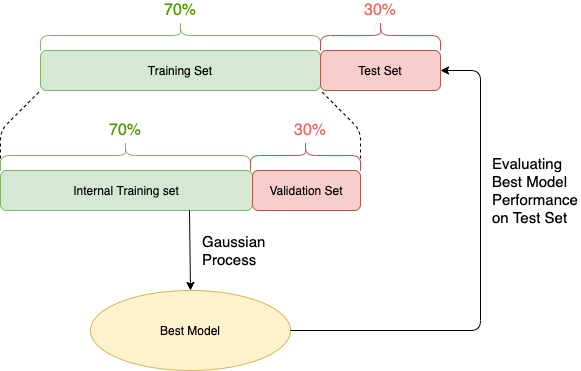
\includegraphics[width=0.9\textwidth]{train_test_scheme.png}
\caption{Single internal and external holdouts process diagram. Note that this
process is repeated 10 times.} 
\label{fig:train_test_diagram}
\end{figure}
In order to train both single-task and multi-task models, we used the data described in Section~\ref{sec:epigenomic_data}. The features are filtered using the selection methods described earlier (see Section~\ref{sec:featureselection}). In Appendix~\ref{appendix:features_tables} are reported the tables containing the selected features. 
Furthermore, for both models, we tried to use both an unbalanced and balanced configurations of training and test sets. 

\section{Single-Task Neural Network Architecture} 
\label{sec:exp_setup_singletask}
% single task neural network setup
To evaluate the performance of multi-task neural networks, we need to consider a benchmark model in our experimental setup. Due to their excellent results, obtained in the context of CRRs classification \cite{WassermannDECRES}, we choose to use a classical feed-forward neural network (explained in Section~\ref{sec:singletaskNN}). Fixed a computational task $p$, the network takes the reduced set of epigenetic features as input and give the prediction of the labels $Y$. A Gaussian process performs the model search, the models can have from no hidden layers up to three hidden layers. In Table~\ref{tab:mlp_single_arch} are reported the number of neurons search space for every layer of the network. Since we have seen in previous experiments that pyramidal architecture networks give better performances the bayesian optimizer is always forced to select an architecture such as the neurons of layer $i$ are greater or equals to the neurons of layer $i+1$. 
A slight variation of SGD explained in Section~\ref{sec:singletaskNN} called Stochastic Gradient Descend with momentum is employed to optimize the weights of the network. The initial learning rate, the $\ell_2$-regularization amount to control model complexity, and the momentum to stabilize the optimization are set respectively to 0.3, 0.001 and 0.5. The training set is iterated for 1000 epochs maximum, and the learning rate could be reduced as the number of iterations increases with a rate of 0.01. Finally, the batch size is fixed at 100 samples per batch.  
\begin{table}[t]
\centering
\begin{tabular}{lll}
\toprule
\textbf{Layer} & \textbf{Neurons} & \textbf{Activation} \\ 
\midrule
1 & (2, 4, 8, 16, 32, 64, 128, 256) & ReLU \\ 
2 & (2, 4, 8, 16, 32, 64, 128) & ReLU \\ 
3 & (2, 4, 8, 16, 32, 64) & ReLU \\ 
4 & 1 & Sigmoid \\ 
\bottomrule
\end{tabular}
\caption{Parameters setting for single-task feed-forward neural network}
\label{tab:mlp_single_arch}
\end{table}

The code implementing the single-task experiments was originally developed in University of Milan by a Computational Biology and Bioinformatics laboratory (Anacleto Lab) research group in order to evaluate the ability of neural network to distinguish cis-regulatory regions. During this works some of those experiments have been repeated and the results are discussed in Section~\ref{sec:single_results}. 

\section{Multi-Task neural network architecture} \label{sec:exp_setup_multitask}
% multi task neural network setup
We choose to use an hard parameters sharing architecture explained in Section~\ref{sec:MTLsection}. The model is constructed with a multi-input and multi-output setting. There is an input branch for every features sets $F_\ell$ and an output branch for every cell lines. The main body of hidden layer connect input branches with output branches. Summarizing the architecture is divided in the following three main parts:
\begin{itemize}
    \item \textit{input branches layers}: every $F_\ell$ will be taken in input by a different branch of hidden layers;
    \item \textit{main body}: it is composed by shared hidden layers. These hidden layers aim to share knowledge between cell lines. The prediction on a particular line $\ell$ could be affected by the information given from the other ones;
    \item \textit{output branches layers}: the main body is split in different branches of hidden layers. Their purpose is giving the predictions of labels $Y$ of every $\ell \in L$.
\end{itemize}
In Figure~\ref{fig:MTL_arch_diagram} we report a diagram of the used architecture.
\begin{figure}[ht]
\centering
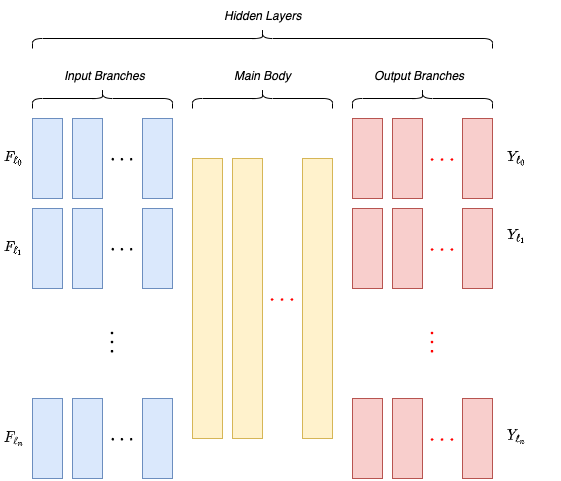
\includegraphics[width=\textwidth]{MTL_diagram.png}
\caption{Multi-tasks neural network architecture. On the left, every input branch takes a cell lines feature set, on the right, every output branch give the predictions for every cell line $\ell$. They are connected, in the middle, by the main body layers. } 
\label{fig:MTL_arch_diagram}
\end{figure}
Note that the network could have the input or the output directly connected to the main body without any input or output layers. 
Also in this case the models search is performed by the Gaussian Process
(Section~\ref{sec:gaussianprocess}). The input branches, output branches and
the main body can have from zero up to three layers. In Table~\ref{tab:mplmtl} are summarized the number of neurons search space for every part of the network. 
To train the models, a Stochastic Gradient Descent with momentum algorithm is used. The initial learning rate is chosen by Gaussian optimizer in a range between 0.1 and 0.2 and it decays with the increasing of iterations with a 0.01 rate. The momentum and the dropout (a form of model complexity control) are set respectively to 0.5 and 0.2. Also in this case the model is iterated for 1000 epochs, the batch size is fixed to 1000 sample per batch. 
\begin{table}[t]
\centering
\begin{tabular}{llll}
\toprule
\textbf{Arch. Parts} & \textbf{Layers} & \textbf{Neurons per Layer} & \textbf{Activation} \\ 
\midrule
\multirow{2}{*}{\textit{Input branch}}  & 1 & 64, 128, 256, 512 & ReLU \\ 
{} & 2 & 32, 64, 128, 256, 512 & ReLU \\
{} & 3 & 16, 32, 64, 128, 256, 512 & ReLU \\
\midrule
\multirow{2}{*}{\textit{main body}} & 1 & 2, 4, 8, 16, 32, 64, 128, 256, 512 & ReLU \\ 
{} & 2 & 2, 4, 8, 16, 32, 64, 128, 512 & ReLU \\
{} & 3 & 2, 4, 8, 16, 32, 64, 128, 256, 512 & ReLU \\
\midrule
\multirow{2}{*}{\textit{output branch}} & 1 & 2, 4, 8, 16, 32, 64, 128, 256, 512 & ReLU\\ 
{} & 2 & 2, 4, 8, 16, 32, 64, 128, 256, 512 & ReLU \\
{} & 3 & 2, 4, 8, 16, 32, 64, 128, 256, 512 & Sigmoid \\
\bottomrule
\end{tabular}
\caption{Parameters setting for multi-task neural network}
\label{tab:mplmtl}
\end{table}
For all of the three parts just described we tried two neurons size configurations. In the former we constrained the Gaussian process to keep a fixed number of neurons for every layer, in the latter, instead, for every neural network section (input branches, main body, output branches) the optimizer selects a pyramidal structure where the neurons of layer $i$ are greater or equals to the neurons of layer $i+1$.
In Section~\ref{sec:multi_results} we reported the results obtained from the various experiments configurations. 

The code implementing these experiments has been developed by the authors of this work in a joint collaboration between the Laboratory for Web Algorithmics (LAW) and Computational Biology and Bioinformatics laboratory (Anacleto Lab) in University of Milan. This code is available on Github\footnote{\url{https://github.com/lipry/MultiTaskLearningExperiments}}. The obtained results are discussed in Section~\ref{sec:multi_results}.

